\documentclass[compress, 8pt, aspectratio=169]{beamer}

\usepackage{presentationtemplate}
\usepackage[fontsize=\small,linenosfontsize=\tiny,askip=3mm]
  {mylisting}
\usepackage[fontsize=\small,askip=3mm]{terminal}
\usepackage{textcomp}
\usepackage[autostyle=true]{csquotes}

\usetikzlibrary{calc}

\title{Conan}

\newcommand{\conandoc}{https://docs.conan.io/2}

% Literal "!" inside a terminal: every single "!" toggles the
% minted escape state, so a literal exclamation mark must be
% emitted through a macro call inside a proper escape region
% (write !\excl!); the macro name must not contain "!"
\newcommand{\excl}{!}

\makeatletter
\newdimen\cn@FVleftmargin
\let\cn@FVSetupFont\FV@SetupFont
\def\FV@SetupFont{%
  \cn@FVleftmargin=\leftmargin
  \cn@FVSetupFont
  \let\leftmargin\cn@FVleftmargin}
\makeatother

\begin{document}

\begin{frame}
  \titlepage
\end{frame}

\begin{frame}{Пакетные менеджеры}

  Задачи пакетного менеджера:

  \bigbreak

  \begin{itemize}

    \item выбрать совместимые версии зависимостей (построить граф зависимостей);

    \item обеспечить доставку зависимостей (скачать исходники и собрать или скачать готовые бинарники);

    \item обеспечить повторяемость сборки;

    \item делиться бинарниками между разработчиками и CI.

  \end{itemize}

\end{frame}

\begin{frame}{Пакетные менеджеры}

  \begin{center}

    \renewcommand{\arraystretch}{1.5}

    \begin{tabular}{|p{2.0cm}|p{4.6cm}|p{4.4cm}|}

      \hline

      \textbf{Логотип} & \textbf{Пакетный менеджер}
        & \textbf{Экосистема} \\

      \hline

      
\includegraphics[height=0.2cm]
        {presentations/images/npm-logo.png}
        & npm & JavaScript/Node.js \\

      
\includegraphics[height=0.4cm]
        {presentations/images/pypi-logo.png}
        & pip & Python \\

      
\includegraphics[height=0.4cm]
        {presentations/images/cargo-logo.png}
        & Cargo & Rust \\

      
\includegraphics[height=0.3cm]
        {presentations/images/nuget-logo.png}
        & NuGet & .NET \\

      
\includegraphics[height=0.2cm]
        {presentations/images/maven-logo.png}
        & Maven & Java \\

      \hline

    \end{tabular}

  \end{center}

\end{frame}

\begin{frame}{О Conan}

  \begin{itemize}

    \item открытый пакетный менеджер C/C++, лицензия MIT;

    \item один из основных C/C++-менеджеров наряду с vcpkg
      (Microsoft);

    \item написан на Python;

    \item 3.6 млн загрузок с PyPI в месяц;

    \item проект появился в 2015 г., активно развивается в JFrog;

    \item Conan 2.0\footnotemark{}%
      \footnotetext{\url{\conandoc/knowledge/whatsnew.html}} вышел в феврале 2023.

  \end{itemize}

\end{frame}

\begin{frame}{Ресурсы}

  \begin{itemize}

    \item Tutorial\footnotemark{}\footnotetext{\url{\conandoc/tutorial.html}};

    \item Reference\footnotemark{}\footnotetext{\url{\conandoc/reference.html}};

    \item Conancenter\footnotemark{}\footnotetext{\url{https://conan.io/center}}
      (\~2000 рецептов, более 10000 версий, данные на 11/2026);

    \item GitHub\footnotemark{}\footnotetext{\url{https://github.com/conan-io/conan}}.

  \end{itemize}

\end{frame}

\begin{frame}[fragile]{Базовые понятия}

  \begin{center}

    \begin{tikzpicture}[
      box/.style={draw, thick, align=center, inner sep=4pt,
        font=\footnotesize}, arr/.style={->, thick}
    ]
      \node (recipe) {
        
\includegraphics[width=1cm]
          {presentations/images/source_code.png}
      };
      \node [above=0mm of recipe] { Рецепт };

      \matrix (sources) [below left=1cm and 2cm of recipe, column sep=0.1cm] {
        \node (src1) {
          
\includegraphics[width=1cm]
            {presentations/images/source_code.png}
        };
&
        \node (src2) {
          
\includegraphics[width=1cm]
            {presentations/images/source_code.png}
        };
\\
      };
      \node [below=0mm of sources] { Исходники };

      \matrix (profiles) [below=1.5cm of recipe, column sep=0.1cm] {
        \node (profile1) {
          
\includegraphics[width=1cm]
            {presentations/images/source_code.png}
        };
&
        \node (profile2) {
          
\includegraphics[width=1cm]
            {presentations/images/source_code.png}
        };
\\
      };
      \node [below=0mm of profiles] { Профили };

      \matrix (packages) [below right=1cm and 2cm of recipe, column sep=0.1cm] {
        \node (pkg1) {
          
\includegraphics[width=1cm]
            {presentations/images/binary-file.png}
        };
&
        \node (pkg2) {
          
\includegraphics[width=1cm]
            {presentations/images/binary-file.png}
        };
\\
      };
      \node [below=0mm of packages] { Пакеты };

      \draw[arr] (sources.north east) -- (recipe.south west);
      \draw[arr] (profiles.north) -- (recipe.south);
      \draw[arr] (recipe.south east) -- (packages.north west);

    \end{tikzpicture}

  \end{center}

\end{frame}

\begin{frame}[fragile]{conanfile.txt\footnotemark{}}

  \myinputlisting[minted language=ini]
    {presentations/03-conan/src/}
    {01-basic/conanfile.txt}

  \bigbreak

  \begin{itemize}

    \item \texttt{[requires]} --- что нужно проекту;

    \item \texttt{[generators]} --- что сгенерировать под
      сборочную систему;

    \item \texttt{[layout]} --- куда раскладывать сгенерированные
      файлы.

  \end{itemize}

  \footnotetext{\url{\conandoc/reference/conanfile_txt.html}}

\end{frame}

\begin{frame}[fragile]{conan install}

  {\small
  \begin{terminalwindow}[!!][minted options={escapeinside=!!, lastline=20}]
!\shellcommand{cd src/01-basic}!
!\shellcommand{conan install . --build=missing}!
======== Input profiles ========
Profile host:
[settings]
arch=x86_64
build_type=Release
compiler=gcc
compiler.cppstd=gnu17
compiler.libcxx=libstdc++11
compiler.version=15
os=Linux

Profile build:
[settings]
!\dots!
======== Computing dependency graph ========
zlib/1.3.1: Not found in local cache, looking in remotes!\dots!
zlib/1.3.1: Checking remote: conancenter
Connecting to remote 'conancenter' anonymously
zlib/1.3.1: Downloaded recipe revision cac0f6!\dots!
Graph root
    conanfile.txt: !\dots!/01-basic/conanfile.txt
Requirements
    zlib/1.3.1#cac0f6!\dots! - Downloaded (conancenter)

======== Computing necessary packages ========
Requirements
    zlib/1.3.1#cac0f6!\dots!:5172!\dots!6625 - Build

======== Installing packages ========
zlib/1.3.1: Building from source
zlib/1.3.1: settings: os=Linux arch=x86_64 compiler=gcc compiler.version=15 build_type=Release
zlib/1.3.1: options: fPIC=True shared=False
!\dots!
-- The C compiler identification is GNU 15.3.0
!\dots!
[ 93%] Building C object CMakeFiles/zlib.dir/zutil.c.o
[100%] Linking C static library libz.a
[100%] Built target zlib
!\dots!
zlib/1.3.1: package(): Packaged 2 '.h' files: zlib.h, zconf.h
zlib/1.3.1: package(): Packaged 1 '.a' file: libz.a
zlib/1.3.1: package(): Packaged 1 file: LICENSE
zlib/1.3.1: Created package revision b6c21644!\dots!
zlib/1.3.1: Package '5172!\dots!6625' created

======== Finalizing install (deploy, generators) ========
!\dots!
conanfile.txt: CMakeDeps necessary find_package() and targets for your CMakeLists.txt
    find_package(ZLIB)
    target_link_libraries(!\dots! ZLIB::ZLIB)
!\dots!
Install finished successfully
  \end{terminalwindow}
  }

  \textit{To be continued \dots}

\end{frame}

\begin{frame}[fragile]{conan install}

  \textit{\dots continued}\bigbreak

  {\small
  \begin{terminalwindow}[!!][minted options={escapeinside=!!, firstline=21, lastline=40}]
!\shellcommand{cd src/01-basic}!
!\shellcommand{conan install . --build=missing}!
======== Input profiles ========
Profile host:
[settings]
arch=x86_64
build_type=Release
compiler=gcc
compiler.cppstd=gnu17
compiler.libcxx=libstdc++11
compiler.version=15
os=Linux

Profile build:
[settings]
!\dots!
======== Computing dependency graph ========
zlib/1.3.1: Not found in local cache, looking in remotes!\dots!
zlib/1.3.1: Checking remote: conancenter
Connecting to remote 'conancenter' anonymously
zlib/1.3.1: Downloaded recipe revision cac0f6!\dots!
Graph root
    conanfile.txt: !\dots!/01-basic/conanfile.txt
Requirements
    zlib/1.3.1#cac0f6!\dots! - Downloaded (conancenter)

======== Computing necessary packages ========
Requirements
    zlib/1.3.1#cac0f6!\dots!:5172!\dots!6625 - Build

======== Installing packages ========
zlib/1.3.1: Building from source
zlib/1.3.1: settings: os=Linux arch=x86_64 compiler=gcc compiler.version=15 build_type=Release
zlib/1.3.1: options: fPIC=True shared=False
!\dots!
-- The C compiler identification is GNU 15.3.0
!\dots!
[ 93%] Building C object CMakeFiles/zlib.dir/zutil.c.o
[100%] Linking C static library libz.a
[100%] Built target zlib
!\dots!
zlib/1.3.1: package(): Packaged 2 '.h' files: zlib.h, zconf.h
zlib/1.3.1: package(): Packaged 1 '.a' file: libz.a
zlib/1.3.1: package(): Packaged 1 file: LICENSE
zlib/1.3.1: Created package revision b6c21644!\dots!
zlib/1.3.1: Package '5172!\dots!6625' created

======== Finalizing install (deploy, generators) ========
!\dots!
conanfile.txt: CMakeDeps necessary find_package() and targets for your CMakeLists.txt
    find_package(ZLIB)
    target_link_libraries(!\dots! ZLIB::ZLIB)
!\dots!
Install finished successfully
  \end{terminalwindow}
  }

  \textit{To be continued \dots}

\end{frame}

\begin{frame}[fragile]{conan install}

  \textit{\dots continued}\bigbreak

  {\small
  \begin{terminalwindow}[!!][minted options={escapeinside=!!, firstline=41}]
!\shellcommand{cd src/01-basic}!
!\shellcommand{conan install . --build=missing}!
======== Input profiles ========
Profile host:
[settings]
arch=x86_64
build_type=Release
compiler=gcc
compiler.cppstd=gnu17
compiler.libcxx=libstdc++11
compiler.version=15
os=Linux

Profile build:
[settings]
!\dots!
======== Computing dependency graph ========
zlib/1.3.1: Not found in local cache, looking in remotes!\dots!
zlib/1.3.1: Checking remote: conancenter
Connecting to remote 'conancenter' anonymously
zlib/1.3.1: Downloaded recipe revision cac0f6!\dots!
Graph root
    conanfile.txt: !\dots!/01-basic/conanfile.txt
Requirements
    zlib/1.3.1#cac0f6!\dots! - Downloaded (conancenter)

======== Computing necessary packages ========
Requirements
    zlib/1.3.1#cac0f6!\dots!:5172!\dots!6625 - Build

======== Installing packages ========
zlib/1.3.1: Building from source
zlib/1.3.1: settings: os=Linux arch=x86_64 compiler=gcc compiler.version=15 build_type=Release
zlib/1.3.1: options: fPIC=True shared=False
!\dots!
-- The C compiler identification is GNU 15.3.0
!\dots!
[ 93%] Building C object CMakeFiles/zlib.dir/zutil.c.o
[100%] Linking C static library libz.a
[100%] Built target zlib
!\dots!
zlib/1.3.1: package(): Packaged 2 '.h' files: zlib.h, zconf.h
zlib/1.3.1: package(): Packaged 1 '.a' file: libz.a
zlib/1.3.1: package(): Packaged 1 file: LICENSE
zlib/1.3.1: Created package revision b6c21644!\dots!
zlib/1.3.1: Package '5172!\dots!6625' created

======== Finalizing install (deploy, generators) ========
!\dots!
conanfile.txt: CMakeDeps necessary find_package() and targets for your CMakeLists.txt
    find_package(ZLIB)
    target_link_libraries(!\dots! ZLIB::ZLIB)
!\dots!
Install finished successfully
  \end{terminalwindow}
  }

\end{frame}

\begin{frame}{Где хранятся зависимости}

  \begin{itemize}

    \item Conancenter\footnotemark{}\footnotetext{\url{https://conan.io/center}}:
      публичный репозиторий рецептов\footnotemark{}%
      \footnotetext{\url{https://github.com/conan-io/conan-center-index}}
      и готовых бинарников;

    \item бинарники хранятся в локальном кэше
      \texttt{\textasciitilde/.conan2};

    \item можно поднять свой сервер с репозиторием пакетов Conan.

  \end{itemize}

\end{frame}

\begin{frame}[fragile]{Версионные диапазоны}

  \myinputlisting[minted language=ini]
    {presentations/03-conan/src/}
    {02-version-range/conanfile.txt}

  \bigbreak

  \begin{itemize}

    \item диапазон разрешается в максимальную доступную версию;

    \item по умолчанию разрешение идёт по локальному кэшу (без удаленного
      репозитория);

    \item с \texttt{--update} проверяется remote;

    \item конкретную версию можно узнать при вычислении графа.

  \end{itemize}

\end{frame}

\begin{frame}[fragile]{[tool\_requires] и [test\_requires]\footnotemark{}}

  \myinputlisting[minted language=ini]
    {presentations/03-conan/src/}
    {03-tool-requires/conanfile.txt}

  \bigbreak

  \begin{itemize}

    \item \texttt{[requires]} --- хост-зависимости (линкуются в
      продукт);

    \item \texttt{[tool\_requires]} --- инструменты для сборки
      (build-контекст), в продукт не линкуются;

    \item \texttt{[test\_requires]} --- зависимости для тестов
      (используются в \texttt{test\_package}).

  \end{itemize}

  \footnotetext{\url{\conandoc/reference/conanfile/attributes.html}}

\end{frame}

\begin{frame}[fragile]{Граф и контексты}

  {\small
  \begin{terminalwindow}[!!][minted options={escapeinside=!!, lastline=17}]
!\shellcommand{cd src/03-tool-requires}!
!\shellcommand{conan graph info .}!
!\dots!
zstd/1.5.7: Not found in local cache, looking in remotes!\dots!
zstd/1.5.7: Checking remote: conancenter
Connecting to remote 'conancenter' anonymously
zstd/1.5.7: Downloaded recipe revision b68ca8!\dots!
cmake/4.5.0: Not found in local cache, looking in remotes!\dots!
cmake/4.5.0: Checking remote: conancenter
cmake/4.5.0: Downloaded recipe revision 24bd34!\dots!
gtest/1.18.0: Not found in local cache, looking in remotes!\dots!
gtest/1.18.0: Checking remote: conancenter
gtest/1.18.0: Downloaded recipe revision e2507f!\dots!
Graph root
    conanfile.txt: !\dots!/03-tool-requires/conanfile.txt
Requirements
    zstd/1.5.7#b68ca8!\dots! - Downloaded (conancenter)
Test requirements
    gtest/1.18.0#e2507f!\dots! - Downloaded (conancenter)
Build requirements
    cmake/4.5.0#24bd34!\dots! - Downloaded (conancenter)
Resolved version ranges
    cmake/[>=3.16]: cmake/4.5.0

======== Computing necessary packages ========
Requirements
    zstd/1.5.7#b68ca8!\dots!:bf9a53!\dots! - Missing
Test requirements
    gtest/1.18.0#e2507f!\dots!:75d8f4!\dots! - Missing
Build requirements
    cmake/4.5.0#24bd34!\dots!:63fead!\dots!#8cf086!\dots! - Download (conancenter)

-------- Basic graph information --------
!\dots!
WARN: There are some error(s) in the graph:
    - Missing packages: gtest, zstd
  \end{terminalwindow}
  }

  \textit{To be continued \dots}

\end{frame}

\begin{frame}[fragile]{Граф и контексты}

  \textit{\dots continued}\bigbreak

  {\small
  \begin{terminalwindow}[!!][minted options={escapeinside=!!, firstline=18, lastline=32}]
!\shellcommand{cd src/03-tool-requires}!
!\shellcommand{conan graph info .}!
!\dots!
zstd/1.5.7: Not found in local cache, looking in remotes!\dots!
zstd/1.5.7: Checking remote: conancenter
Connecting to remote 'conancenter' anonymously
zstd/1.5.7: Downloaded recipe revision b68ca8!\dots!
cmake/4.5.0: Not found in local cache, looking in remotes!\dots!
cmake/4.5.0: Checking remote: conancenter
cmake/4.5.0: Downloaded recipe revision 24bd34!\dots!
gtest/1.18.0: Not found in local cache, looking in remotes!\dots!
gtest/1.18.0: Checking remote: conancenter
gtest/1.18.0: Downloaded recipe revision e2507f!\dots!
Graph root
    conanfile.txt: !\dots!/03-tool-requires/conanfile.txt
Requirements
    zstd/1.5.7#b68ca8!\dots! - Downloaded (conancenter)
Test requirements
    gtest/1.18.0#e2507f!\dots! - Downloaded (conancenter)
Build requirements
    cmake/4.5.0#24bd34!\dots! - Downloaded (conancenter)
Resolved version ranges
    cmake/[>=3.16]: cmake/4.5.0

======== Computing necessary packages ========
Requirements
    zstd/1.5.7#b68ca8!\dots!:bf9a53!\dots! - Missing
Test requirements
    gtest/1.18.0#e2507f!\dots!:75d8f4!\dots! - Missing
Build requirements
    cmake/4.5.0#24bd34!\dots!:63fead!\dots!#8cf086!\dots! - Download (conancenter)

-------- Basic graph information --------
!\dots!
WARN: There are some error(s) in the graph:
    - Missing packages: gtest, zstd
  \end{terminalwindow}
  }

  \textit{To be continued \dots}

\end{frame}

\begin{frame}[fragile]{Граф и контексты}

  \textit{\dots continued}\bigbreak

  {\small
  \begin{terminalwindow}[!!][minted options={escapeinside=!!, firstline=33}]
!\shellcommand{cd src/03-tool-requires}!
!\shellcommand{conan graph info .}!
!\dots!
zstd/1.5.7: Not found in local cache, looking in remotes!\dots!
zstd/1.5.7: Checking remote: conancenter
Connecting to remote 'conancenter' anonymously
zstd/1.5.7: Downloaded recipe revision b68ca8!\dots!
cmake/4.5.0: Not found in local cache, looking in remotes!\dots!
cmake/4.5.0: Checking remote: conancenter
cmake/4.5.0: Downloaded recipe revision 24bd34!\dots!
gtest/1.18.0: Not found in local cache, looking in remotes!\dots!
gtest/1.18.0: Checking remote: conancenter
gtest/1.18.0: Downloaded recipe revision e2507f!\dots!
Graph root
    conanfile.txt: !\dots!/03-tool-requires/conanfile.txt
Requirements
    zstd/1.5.7#b68ca8!\dots! - Downloaded (conancenter)
Test requirements
    gtest/1.18.0#e2507f!\dots! - Downloaded (conancenter)
Build requirements
    cmake/4.5.0#24bd34!\dots! - Downloaded (conancenter)
Resolved version ranges
    cmake/[>=3.16]: cmake/4.5.0

======== Computing necessary packages ========
Requirements
    zstd/1.5.7#b68ca8!\dots!:bf9a53!\dots! - Missing
Test requirements
    gtest/1.18.0#e2507f!\dots!:75d8f4!\dots! - Missing
Build requirements
    cmake/4.5.0#24bd34!\dots!:63fead!\dots!#8cf086!\dots! - Download (conancenter)

-------- Basic graph information --------
!\dots!
WARN: There are some error(s) in the graph:
    - Missing packages: gtest, zstd
  \end{terminalwindow}
  }

  \bigbreak

  \begin{itemize}

    \item у графа три раздела: Requirements (host), Build
      requirements (build), Test requirements (test);

    \item host/build-контексты могут быть разными.

  \end{itemize}

\end{frame}

\begin{frame}[fragile]{Конфликт в графе}

  \myinputlisting[minted language=ini]
    {presentations/03-conan/src/}
    {04-conflict/conanfile.txt}

  \bigbreak

  {\footnotesize
  \begin{terminalwindow}[!!][minted options={escapeinside=!!, lastline=12}]
!\shellcommand{cd src/04-conflict}!
!\shellcommand{conan install .}!
!\dots!
spdlog/1.14.1: Not found in local cache, looking in remotes!\dots!
spdlog/1.14.1: Checking remote: conancenter
Connecting to remote 'conancenter' anonymously
spdlog/1.14.1: Downloaded recipe revision 0c58e5!\dots!
Graph root
    conanfile.txt: !\dots!/04-conflict/conanfile.txt
Requirements
    spdlog/1.14.1#0c58e5!\dots! - Downloaded (conancenter)
ERROR: Version conflict: Conflict between fmt/10.2.1 and fmt/11.2.0 in the graph.
Conflict originates from spdlog/1.14.1

Run 'conan graph info !\dots! --format=html > graph.html' and open 'graph.html' to inspect the conflict graphically.
  \end{terminalwindow}
  }

  \textit{To be continued \dots}

\end{frame}

\begin{frame}[fragile]{Конфликт в графе}

  \textit{\dots continued}\bigbreak

  {\footnotesize
  \begin{terminalwindow}[!!][minted options={escapeinside=!!, firstline=13}]
!\shellcommand{cd src/04-conflict}!
!\shellcommand{conan install .}!
!\dots!
spdlog/1.14.1: Not found in local cache, looking in remotes!\dots!
spdlog/1.14.1: Checking remote: conancenter
Connecting to remote 'conancenter' anonymously
spdlog/1.14.1: Downloaded recipe revision 0c58e5!\dots!
Graph root
    conanfile.txt: !\dots!/04-conflict/conanfile.txt
Requirements
    spdlog/1.14.1#0c58e5!\dots! - Downloaded (conancenter)
ERROR: Version conflict: Conflict between fmt/10.2.1 and fmt/11.2.0 in the graph.
Conflict originates from spdlog/1.14.1

Run 'conan graph info !\dots! --format=html > graph.html' and open 'graph.html' to inspect the conflict graphically.
  \end{terminalwindow}
  }

  \bigbreak

  \begin{itemize}

    \item рецепт \texttt{spdlog/1.14.1} в Conancenter требует
      \texttt{fmt/10.2.1}, а наш \texttt{conanfile} ---
      \texttt{fmt/11.2.0}, версии несовместимы;

    \item Conan не пытается \enquote{угадывать} версию: конфликт виден
      сразу, до сборки;

    \item ошибка называет виновника (\enquote{Conflict originates
      from spdlog/1.14.1}) и подсказывает посмотреть граф в HTML.

  \end{itemize}

\end{frame}

\begin{frame}[fragile]{Граф: html и explain}

  \begin{terminalwindow}
!\shellcommand{cd src/01-basic}!
!\shellcommand{conan graph info . --format=html > /tmp/graph.html}!
!\dots!
======== Computing dependency graph ========
Graph root
    conanfile.txt: !\dots!/01-basic/conanfile.txt
Requirements
    zlib/1.3.1#cac0f6!\dots! - Cache
  \end{terminalwindow}

  \bigbreak

  \begin{itemize}

    \item форматы графа: \texttt{html}, \texttt{json}, \texttt{dot};

    \item \texttt{--format=html} пишет HTML в stdout (поэтому
      \texttt{> graph.html});

    \item \texttt{conan graph explain .}\footnotemark{} объясняет,
      почему бинарник не найден.

  \end{itemize}

  \footnotetext{\url{\conandoc/reference/commands/graph.html}}

\end{frame}

\begin{frame}[fragile]{HTML граф}

  \centering
  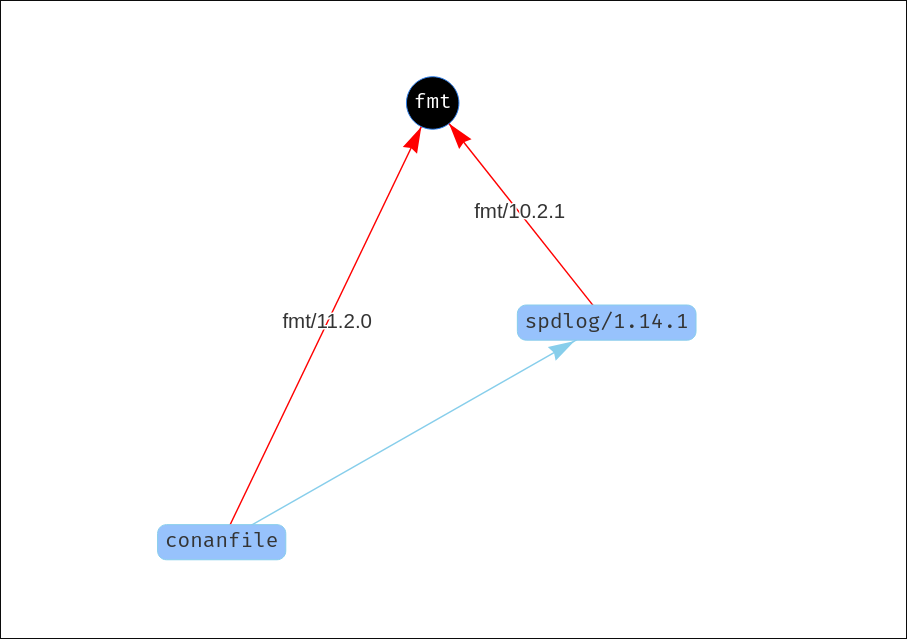
\includegraphics[width=10cm]
    {presentations/03-conan/src/04-conflict/conflict-graph.png}

\end{frame}

\begin{frame}[fragile]{Сгенерированные файлы}

  {\small
  \begin{terminalwindow}[!!][minted options={escapeinside=!!, lastline=14}]
!\shellcommand{cd src/01-basic}!
!\shellcommand{ls build/Release/generators/}!
cmakedeps_macros.cmake
CMakePresets.json
conanbuildenv-release-x86_64.sh
conanbuild.sh
conandeps_legacy.cmake
conanrunenv-release-x86_64.sh
conanrun.sh
conan_toolchain.cmake
deactivate_conanbuildenv-release-x86_64.sh
deactivate_conanbuild.sh
deactivate_conanrun.sh
FindZLIB.cmake
module-ZLIB-release-x86_64-data.cmake
module-ZLIB-Target-release.cmake
module-ZLIBTargets.cmake
ZLIBConfig.cmake
ZLIBConfigVersion.cmake
ZLIB-release-x86_64-data.cmake
ZLIB-Target-release.cmake
ZLIBTargets.cmake
  \end{terminalwindow}
  }

  \textit{To be continued \dots}

\end{frame}

\begin{frame}[fragile]{Сгенерированные файлы}

  \textit{\dots continued}\bigbreak

  {\small
  \begin{terminalwindow}[!!][minted options={escapeinside=!!, firstline=15}]
!\shellcommand{cd src/01-basic}!
!\shellcommand{ls build/Release/generators/}!
cmakedeps_macros.cmake
CMakePresets.json
conanbuildenv-release-x86_64.sh
conanbuild.sh
conandeps_legacy.cmake
conanrunenv-release-x86_64.sh
conanrun.sh
conan_toolchain.cmake
deactivate_conanbuildenv-release-x86_64.sh
deactivate_conanbuild.sh
deactivate_conanrun.sh
FindZLIB.cmake
module-ZLIB-release-x86_64-data.cmake
module-ZLIB-Target-release.cmake
module-ZLIBTargets.cmake
ZLIBConfig.cmake
ZLIBConfigVersion.cmake
ZLIB-release-x86_64-data.cmake
ZLIB-Target-release.cmake
ZLIBTargets.cmake
  \end{terminalwindow}
  }

\end{frame}

\begin{frame}[fragile]{Профили}

  Профили можно генерировать исходя из текущего окружения или создавать
  самостоятельно.

  \begin{columns}[T]

    \column{0.48\textwidth}

    \begin{terminalwindow}
!\shellcommand{conan profile show}!
Host profile:
[settings]
arch=x86_64
build_type=Release
compiler=gcc
compiler.cppstd=gnu17
compiler.libcxx=libstdc++11
compiler.version=15
os=Linux

Build profile:
[settings]
!\dots!
    \end{terminalwindow}

    \column{0.48\textwidth}

    \myinputlisting[minted language=ini]
      {presentations/03-conan/src/}
      {01-basic/profiles/clang}

  \end{columns}

  \bigbreak

\end{frame}

\begin{frame}[fragile]{Профиль в деле}

  {\small
  \begin{terminalwindow}[!!][minted options={escapeinside=!!, lastline=15}]
!\shellcommand{cd src/01-basic}!
!\shellcommand{conan install . -pr ./profiles/clang --build=missing}!
!\dots!
Profile host:
[settings]
arch=x86_64
build_type=Release
compiler=clang
compiler.libcxx=libc++
compiler.version=21
os=Linux
!\dots!
======== Computing necessary packages ========
Connecting to remote 'conancenter' anonymously
Requirements
    zlib/1.3.1#cac0f6!\dots!:1cb0d13b!\dots! - Build

======== Installing packages ========
zlib/1.3.1: Building from source
zlib/1.3.1: settings: os=Linux arch=x86_64 compiler=clang !\dots!
zlib/1.3.1: options: fPIC=True shared=False
!\dots!
-- The C compiler identification is Clang 21.1.8
!\dots!
zlib/1.3.1: Created package revision 3b0d7ec4!\dots!
zlib/1.3.1: Package '1cb0d13b!\dots!' created
Install finished successfully
  \end{terminalwindow}
  }

  \textit{To be continued \dots}

\end{frame}

\begin{frame}[fragile]{Профиль в деле}

  \textit{\dots continued}\bigbreak

  {\small
  \begin{terminalwindow}[!!][minted options={escapeinside=!!, firstline=16}]
!\shellcommand{cd src/01-basic}!
!\shellcommand{conan install . -pr ./profiles/clang --build=missing}!
!\dots!
Profile host:
[settings]
arch=x86_64
build_type=Release
compiler=clang
compiler.libcxx=libc++
compiler.version=21
os=Linux
!\dots!
======== Computing necessary packages ========
Connecting to remote 'conancenter' anonymously
Requirements
    zlib/1.3.1#cac0f6!\dots!:1cb0d13b!\dots! - Build

======== Installing packages ========
zlib/1.3.1: Building from source
zlib/1.3.1: settings: os=Linux arch=x86_64 compiler=clang !\dots!
zlib/1.3.1: options: fPIC=True shared=False
!\dots!
-- The C compiler identification is Clang 21.1.8
!\dots!
zlib/1.3.1: Created package revision 3b0d7ec4!\dots!
zlib/1.3.1: Package '1cb0d13b!\dots!' created
Install finished successfully
  \end{terminalwindow}
  }

\end{frame}

\begin{frame}[fragile]{Кросс-компиляция}

  Три базовые платформы в кросс-компиляции:

  \bigbreak

  \begin{itemize}

    \item \textit{build} --- платформа, на которой выполняется сборка;

    \item \textit{host} --- платформа, на которой будет выполняться
      собираемое приложение;

    \item \textit{target} --- платформа, с машинным кодом которой будет
      работать собираемое приложение\footnotemark{}.

  \end{itemize}

  \footnotetext{Актуально для компиляторов, отладчиков, ассемблеров и т.д.}

\end{frame}

\begin{frame}[fragile]{Кросс-профиль}

  \myinputlisting[minted language=ini]
    {presentations/03-conan/src/}
    {01-basic/profiles/aarch64}

  \bigbreak

  \begin{itemize}

    \item кросс-компиляция: целевая платформа (host) отличается от
      машины сборки (build);

    \item Conan 2 разделяет профили: \texttt{-pr:h} (host) и
      \texttt{-pr:b} (build).

  \end{itemize}

\end{frame}

\begin{frame}[fragile]{Как не надо писать CMake}

  Зашитый компилятор и флаги не дают подменить компилятор, заданный в профиле.

  \bigbreak

  \myinputlisting[minted language=cmake]
    {presentations/03-conan/src/}
    {01-basic/bad/CMakeLists.txt}

\end{frame}

\begin{frame}[fragile]{\texttt{[buildenv]} и \texttt{[conf]}}

  Профили позволяют задавать переменные окружения сборочной среды и некоторые
  настройки сборочных систем.
  Также поддерживается включение других профилей для их
  дополнения/переопределения.

  \begin{columns}[T]

    \column{0.48\textwidth}

    \myinputlisting[minted language=ini]
      {presentations/03-conan/src/}
      {01-basic/profiles/buildenv}

    \column{0.48\textwidth}

    \myinputlisting[minted language=ini]
      {presentations/03-conan/src/}
      {01-basic/profiles/jobs2}

  \end{columns}

\end{frame}

\begin{frame}[fragile]{Окружение из профиля}

  {\small
  \begin{terminalwindow}[!!][minted options={escapeinside=!!, lastline=15}]
!\shellcommand{cd src/01-basic}!
!\shellcommand{conan install . -pr ./profiles/buildenv --build=missing}!
!\dots!
Profile host:
[settings]
arch=x86_64
build_type=Release
compiler=gcc
compiler.version=15
compiler.libcxx=libstdc++11
os=Linux
[buildenv]
CXXFLAGS+=-march=native
!\dots!
======== Computing necessary packages ========
Requirements
    zlib/1.3.1#cac0f6!\dots!:5172!\dots!6625#b6c2!\dots! - Cache
!\dots!
zlib/1.3.1: Already installed!\excl! (1 of 1)
Install finished successfully
!\shellcommand{source build/Release/generators/conanbuild.sh}!
!\shellcommand{echo "CXXFLAGS=[\$CXXFLAGS]"}!
CXXFLAGS=[-march=native]
  \end{terminalwindow}
  }

  \textit{To be continued \dots}

\end{frame}

\begin{frame}[fragile]{Окружение из профиля}

  \textit{\dots continued}\bigbreak

  {\small
  \begin{terminalwindow}[!!][minted options={escapeinside=!!, firstline=16}]
!\shellcommand{cd src/01-basic}!
!\shellcommand{conan install . -pr ./profiles/buildenv --build=missing}!
!\dots!
Profile host:
[settings]
arch=x86_64
build_type=Release
compiler=gcc
compiler.version=15
compiler.libcxx=libstdc++11
os=Linux
[buildenv]
CXXFLAGS+=-march=native
!\dots!
======== Computing necessary packages ========
Requirements
    zlib/1.3.1#cac0f6!\dots!:5172!\dots!6625#b6c2!\dots! - Cache
!\dots!
zlib/1.3.1: Already installed!\excl! (1 of 1)
Install finished successfully
!\shellcommand{source build/Release/generators/conanbuild.sh}!
!\shellcommand{echo "CXXFLAGS=[\$CXXFLAGS]"}!
CXXFLAGS=[-march=native]
  \end{terminalwindow}
  }

\end{frame}

\begin{frame}[fragile]{Первый conanfile.py}

  \begin{columns}[T]

    \column{0.48\textwidth}

    % Фрагмент ступени 1 из src/05-hello/conanfile.py (файл в src/
    % в итоговом состоянии, менять нельзя --- hence in-place)
    \begin{myinplacelisting}[minted language=python]
from conan import ConanFile


class HelloConan(ConanFile):
    name = "hello"
    version = "0.1.0"
    settings = "os", "arch", "compiler",
      "build_type"
    \end{myinplacelisting}

    \column{0.48\textwidth}

    \begin{mytitledinplacelisting}[minted language=text]{05-hello/}
05-hello/
├── CMakeLists.txt
├── conanfile.py
├── include/
│   └── hello/
│       └── hello.hpp
├── src/
│   └── hello.cpp
└── test_package/
    ├── CMakeLists.txt
    ├── conanfile.py
    └── src/
        └── test.cpp
    \end{mytitledinplacelisting}

  \end{columns}

\end{frame}

\begin{frame}[fragile]{Первый conanfile.py}

  \myinputlisting[minted language=cmake]
    {presentations/03-conan/src/}
    {05-hello/CMakeLists.txt}

  \bigbreak

\end{frame}

\begin{frame}[fragile]{Код пакета}

  \begin{columns}[T]

    \column{0.48\textwidth}

    \myinputlisting[minted language=c++]
      {presentations/03-conan/src/}
      {05-hello/include/hello/hello.hpp}

    \bigbreak

    \myinputlisting[minted language=c++]
      {presentations/03-conan/src/}
      {05-hello/src/hello.cpp}

    \column{0.48\textwidth}

    \myinputlisting[minted language=c++]
      {presentations/03-conan/src/}
      {05-hello/test_package/src/test.cpp}

  \end{columns}

\end{frame}

\begin{frame}[fragile]{\texttt{generate()}}

  % Фрагмент ступени 2 из src/05-hello/conanfile.py (in-place:
  % ступень не существует как отдельный файл)
  \begin{myinplacelisting}[minted language=python]
from conan.tools.cmake import CMake, CMakeToolchain, CMakeDeps, cmake_layout
from conan import ConanFile


class HelloConan(ConanFile):
  |\dots|
    def layout(self):
        cmake_layout(self)

    def generate(self):
        tc = CMakeToolchain(self)
        tc.generate()
        deps = CMakeDeps(self)
        deps.generate()
  \end{myinplacelisting}

\end{frame}

\begin{frame}[fragile]{\texttt{generate()}}

  {\small
  \begin{terminalwindow}[!!][minted options={escapeinside=!!, lastline=11}]
!\shellcommand{cd src/05-hello}!
!\shellcommand{conan install .}!
!\dots!
conanfile.py (hello/0.1.0): Calling generate()
conanfile.py (hello/0.1.0): Generators folder: !\dots!/05-hello/build/Release/generators
conanfile.py (hello/0.1.0): CMakeToolchain generated: conan_toolchain.cmake
conanfile.py (hello/0.1.0): CMakeToolchain: Preset 'conan-release' added to CMakePresets.json.
    (cmake>=3.23) cmake --preset conan-release
    (cmake<3.23) cmake <path> -G "Unix Makefiles" -DCMAKE_TOOLCHAIN_FILE=!\dots!
!\dots!
Install finished successfully
!\shellcommand{cmake -S . -B build/Release -C build/Release/generators/conan\_toolchain.cmake}!
loading initial cache file build/Release/generators/conan_toolchain.cmake
-- Using Conan toolchain: !\dots!/05-hello/build/Release/generators/conan_toolchain.cmake
-- Conan toolchain: Setting CMAKE_POSITION_INDEPENDENT_CODE=ON (options.fPIC)
-- Conan toolchain: Defining architecture flag: -m64
-- Conan toolchain: C++ Standard 17 with extensions ON
-- Conan toolchain: Setting BUILD_SHARED_LIBS = OFF
!\dots!
-- Configuring done (0.0s)
-- Generating done (0.0s)
-- Build files have been written to: !\dots!/05-hello/build/Release
  \end{terminalwindow}
  }

  \textit{To be continued \dots}

\end{frame}

\begin{frame}[fragile]{\texttt{generate()}}

  \textit{\dots continued}\bigbreak

  {\small
  \begin{terminalwindow}[!!][minted options={escapeinside=!!, firstline=12}]
!\shellcommand{cd src/05-hello}!
!\shellcommand{conan install .}!
!\dots!
conanfile.py (hello/0.1.0): Calling generate()
conanfile.py (hello/0.1.0): Generators folder: !\dots!/05-hello/build/Release/generators
conanfile.py (hello/0.1.0): CMakeToolchain generated: conan_toolchain.cmake
conanfile.py (hello/0.1.0): CMakeToolchain: Preset 'conan-release' added to CMakePresets.json.
    (cmake>=3.23) cmake --preset conan-release
    (cmake<3.23) cmake <path> -G "Unix Makefiles" -DCMAKE_TOOLCHAIN_FILE=!\dots!
!\dots!
Install finished successfully
!\shellcommand{cmake -S . -B build/Release -C build/Release/generators/conan\_toolchain.cmake}!
loading initial cache file build/Release/generators/conan_toolchain.cmake
-- Using Conan toolchain: !\dots!/05-hello/build/Release/generators/conan_toolchain.cmake
-- Conan toolchain: Setting CMAKE_POSITION_INDEPENDENT_CODE=ON (options.fPIC)
-- Conan toolchain: Defining architecture flag: -m64
-- Conan toolchain: C++ Standard 17 with extensions ON
-- Conan toolchain: Setting BUILD_SHARED_LIBS = OFF
!\dots!
-- Configuring done (0.0s)
-- Generating done (0.0s)
-- Build files have been written to: !\dots!/05-hello/build/Release
  \end{terminalwindow}
  }

\end{frame}

\begin{frame}[fragile]{\texttt{build()}}

  % Фрагмент ступени 3 из src/05-hello/conanfile.py (in-place:
  % файл в src/ в итоговом состоянии)
  \begin{myinplacelisting}[minted language=python]
|\dots|

class HelloConan(ConanFile):
|\dots|
    def build(self):
        cmake = CMake(self)
        cmake.configure()
        cmake.build()
  \end{myinplacelisting}

  \bigbreak

  {\small
  \begin{terminalwindow}[!!][minted options={escapeinside=!!, lastline=10}]
!\shellcommand{rm -rf build}!
!\shellcommand{conan build .}!
!\dots!
conanfile.py (hello/0.1.0): Calling build()
conanfile.py (hello/0.1.0): Running CMake.configure()
conanfile.py (hello/0.1.0): RUN: cmake -G "Unix Makefiles"\\
-DCMAKE_TOOLCHAIN_FILE="generators/conan_toolchain.cmake"
-DCMAKE_INSTALL_PREFIX=!\dots!\\
-DCMAKE_POLICY_DEFAULT_CMP0091="NEW"
-DCMAKE_BUILD_TYPE="Release" "!\dots!"
-- Using Conan toolchain: !\dots!/05-hello/build/Release/generators/conan_toolchain.cmake
-- Conan toolchain: Setting CMAKE_POSITION_INDEPENDENT_CODE=ON (options.fPIC)
-- Conan toolchain: Defining architecture flag: -m64
-- Conan toolchain: C++ Standard 17 with extensions ON
-- Conan toolchain: Setting BUILD_SHARED_LIBS = OFF
-- The CXX compiler identification is GNU 15.3.0
!\dots!
-- Configuring done (1.1s)
-- Generating done (0.0s)
conanfile.py (hello/0.1.0): Running CMake.build()
[ 50%] Building CXX object CMakeFiles/hello.dir/src/hello.cpp.o
[100%] Linking CXX static library libhello.a
[100%] Built target hello
  \end{terminalwindow}
  }

  \textit{To be continued \dots}

\end{frame}

\begin{frame}[fragile]{\texttt{build()}}

  \textit{\dots continued}\bigbreak

  {\small
  \begin{terminalwindow}[!!][minted options={escapeinside=!!, firstline=11}]
!\shellcommand{rm -rf build}!
!\shellcommand{conan build .}!
!\dots!
conanfile.py (hello/0.1.0): Calling build()
conanfile.py (hello/0.1.0): Running CMake.configure()
conanfile.py (hello/0.1.0): RUN: cmake -G "Unix Makefiles"\\
-DCMAKE_TOOLCHAIN_FILE="generators/conan_toolchain.cmake"
-DCMAKE_INSTALL_PREFIX=!\dots!\\
-DCMAKE_POLICY_DEFAULT_CMP0091="NEW"
-DCMAKE_BUILD_TYPE="Release" "!\dots!"
-- Using Conan toolchain: !\dots!/05-hello/build/Release/generators/conan_toolchain.cmake
-- Conan toolchain: Setting CMAKE_POSITION_INDEPENDENT_CODE=ON (options.fPIC)
-- Conan toolchain: Defining architecture flag: -m64
-- Conan toolchain: C++ Standard 17 with extensions ON
-- Conan toolchain: Setting BUILD_SHARED_LIBS = OFF
-- The CXX compiler identification is GNU 15.3.0
!\dots!
-- Configuring done (1.1s)
-- Generating done (0.0s)
conanfile.py (hello/0.1.0): Running CMake.build()
[ 50%] Building CXX object CMakeFiles/hello.dir/src/hello.cpp.o
[100%] Linking CXX static library libhello.a
[100%] Built target hello
  \end{terminalwindow}
  }

\end{frame}

\begin{frame}[fragile]{Вариант с Meson}

  \myinputlisting[minted language=python,
    minted options={fontsize=\small,breaklines,breakanywhere,
    linenos,numbersep=2pt,lastline=17}]
    {presentations/03-conan/src/}
    {06-hello-meson/conanfile.py}

  \textit{To be continued \dots}

\end{frame}

\begin{frame}[fragile]{Вариант с Meson}

  \textit{\dots continued}\bigbreak

  \myinputlisting[minted language=python,
    minted options={fontsize=\small,breaklines,breakanywhere,
    linenos,numbersep=2pt,firstline=18}]
    {presentations/03-conan/src/}
    {06-hello-meson/conanfile.py}

  \bigbreak

  \myinputlisting[minted language=meson]
    {presentations/03-conan/src/}
    {06-hello-meson/meson.build}

\end{frame}

\begin{frame}[fragile]{\texttt{package()} и \texttt{exports\_sources}}

  % Фрагмент ступени 4 из src/05-hello/conanfile.py (in-place:
  % файл в src/ в итоговом состоянии)
  \begin{myinplacelisting}[minted language=python]
|\dots|

class HelloConan(ConanFile):
    |\dots|
    exports_sources = "CMakeLists.txt", "src/*", "include/*"

    def package(self):
        cmake = CMake(self)
        cmake.install()
  \end{myinplacelisting}

\end{frame}

\begin{frame}[fragile]{conan create}

  {\footnotesize
  \begin{terminalwindow}[!!][minted options={escapeinside=!!, fontsize=\footnotesize, lastline=19}]
!\shellcommand{cd src/05-hello}!
!\shellcommand{conan create .}!
======== Exporting recipe to the cache ========
hello/0.1.0: Exporting package recipe: !\dots!/05-hello/conanfile.py
hello/0.1.0: Copied 1 '.py' file: conanfile.py
hello/0.1.0: Copied 1 '.txt' file: CMakeLists.txt
hello/0.1.0: Copied 1 '.hpp' file: hello.hpp
hello/0.1.0: Copied 1 '.cpp' file: hello.cpp
hello/0.1.0: Exported: hello/0.1.0#70bc0107!\dots! (2026-11-17 20:21:36 UTC)
!\dots!
hello/0.1.0: Forced build from source
Requirements
    hello/0.1.0#70bc0107!\dots!:65f26548!\dots! - Build
!\dots!
hello/0.1.0: Building from source
hello/0.1.0: settings: os=Linux arch=x86_64 compiler=gcc\\
compiler.cppstd=gnu17 compiler.libcxx=libstdc++11 compiler.version=15 build_type=Release
hello/0.1.0: options: fPIC=True shared=False
!\dots!
[ 50%] Building CXX object CMakeFiles/hello.dir/src/hello.cpp.o
[100%] Linking CXX static library libhello.a
  \end{terminalwindow}
  }

  \textit{To be continued \dots}

\end{frame}

\begin{frame}[fragile]{conan create}

  \textit{\dots continued}\bigbreak

  {\footnotesize
  \begin{terminalwindow}[!!][minted options={escapeinside=!!, fontsize=\footnotesize, firstline=20}]
!\shellcommand{cd src/05-hello}!
!\shellcommand{conan create .}!
======== Exporting recipe to the cache ========
hello/0.1.0: Exporting package recipe: !\dots!/05-hello/conanfile.py
hello/0.1.0: Copied 1 '.py' file: conanfile.py
hello/0.1.0: Copied 1 '.txt' file: CMakeLists.txt
hello/0.1.0: Copied 1 '.hpp' file: hello.hpp
hello/0.1.0: Copied 1 '.cpp' file: hello.cpp
hello/0.1.0: Exported: hello/0.1.0#70bc0107!\dots! (2026-11-17 20:21:36 UTC)
!\dots!
hello/0.1.0: Forced build from source
Requirements
    hello/0.1.0#70bc0107!\dots!:65f26548!\dots! - Build
!\dots!
hello/0.1.0: Building from source
hello/0.1.0: settings: os=Linux arch=x86_64 compiler=gcc\\
compiler.cppstd=gnu17 compiler.libcxx=libstdc++11 compiler.version=15 build_type=Release
hello/0.1.0: options: fPIC=True shared=False
!\dots!
[ 50%] Building CXX object CMakeFiles/hello.dir/src/hello.cpp.o
[100%] Linking CXX static library libhello.a
!\dots!
hello/0.1.0: package(): Packaged 1 '.hpp' file: hello.hpp
hello/0.1.0: package(): Packaged 1 '.a' file: libhello.a
hello/0.1.0: Created package revision e9c2246a!\dots!
hello/0.1.0: Package '65f26548!\dots!' created
!\dots!
======== Launching test_package ========
!\dots!
-- Conan: Component target declared 'hello::libhello'
-- Conan: Target declared 'hello::hello'
!\dots!
hello/0.1.0 (test package): RUN: ./test_package
Hello, Conan 2!\excl!
  \end{terminalwindow}
  }

\end{frame}

\begin{frame}[fragile]{conan list}

  {\small
  \begin{terminalwindow}[!!][minted options={escapeinside=!!}]
!\shellcommand{conan list "hello/*:*"}!
Found 1 pkg/version recipes matching hello/* in local cache
Local Cache
  hello
    hello/0.1.0
      revisions
        70bc0107!\dots! (2026-11-17 20:21:36 UTC)
          packages
            65f26548!\dots!
              info
                settings
                  arch: x86_64
                  build_type: Release
                  compiler: gcc
                  compiler.cppstd: gnu17
                  compiler.libcxx: libstdc++11
                  compiler.version: 15
                  os: Linux
                options
                  fPIC: True
                  shared: False
  \end{terminalwindow}
  }

\end{frame}

\begin{frame}[fragile]{Другие атрибуты рецепта}

  % Фрагмент ступени 5 из src/05-hello/conanfile.py (in-place:
  % файл в src/ в итоговом состоянии)
  \begin{myinplacelisting}[minted language=python]
|\dots|

class HelloConan(ConanFile):
    |\dots|
    options = {"shared": [True, False], "fPIC": [True, False]}
    default_options = {"shared": False, "fPIC": True}
    package_type = "library"
  \end{myinplacelisting}

  \bigbreak

  \begin{itemize}

    \item \texttt{options} --- индивидуальные настройки рецепта;

    \item \texttt{package\_type = "library"} --- абстрактный тип:
      конкретный (static/shared-library) Conan выводит из опции
      \texttt{shared};

  \end{itemize}

\end{frame}

\begin{frame}[fragile]{\texttt{package\_info}\footnotemark{}%
  \footnotetext{\url{\conandoc/tutorial/creating_packages/define_package_information.html}}}

  % Фрагмент ступени 6 из src/05-hello/conanfile.py (in-place:
  % файл в src/ в итоговом состоянии)
  \begin{myinplacelisting}[minted language=python]
def package_info(self):
    self.cpp_info.libs = ["hello"]
  \end{myinplacelisting}

  \bigbreak

  \begin{itemize}

    \item \texttt{package\_info()} --- информация о бинарнике для
      потребителя: libs, includedirs, libdirs, requires;

    \item \texttt{libdirs=["lib"]} и \texttt{includedirs=["include"]}
      --- значения по умолчанию, писать не обязательно;

    \item для CMakeDeps из этого автоматически создаётся target
      \texttt{hello::hello} (\texttt{find\_package(hello)}).

  \end{itemize}

\end{frame}

\begin{frame}[fragile]{\texttt{test\_package}\footnotemark{}%
  \footnotetext{\url{\conandoc/tutorial/creating_packages/test_conan_packages.html}}}

  \myinputlisting[minted language=python,
    minted options={fontsize=\small,breaklines,breakanywhere,
    linenos,numbersep=2pt,lastline=14}]
    {presentations/03-conan/src/}
    {05-hello/test_package/conanfile.py}

  \textit{To be continued \dots}

\end{frame}

\begin{frame}[fragile]{\texttt{test\_package}\footnotemark{}%
  \footnotetext{\url{\conandoc/tutorial/creating_packages/test_conan_packages.html}}}

  \textit{\dots continued}\bigbreak

  \myinputlisting[minted language=python,
    minted options={fontsize=\small,breaklines,breakanywhere,
    linenos,numbersep=2pt,firstline=15}]
    {presentations/03-conan/src/}
    {05-hello/test_package/conanfile.py}

  \bigbreak

  % Промежуточный вариант (в src/ итоговый hello::libhello,
  % слайд 40)
  \begin{myinplacelisting}[minted language=cmake]
cmake_minimum_required(VERSION 3.15)
project(test_package CXX)

find_package(hello REQUIRED)

add_executable(test_package src/test.cpp)
target_link_libraries(test_package PRIVATE hello::hello)
  \end{myinplacelisting}

\end{frame}

\begin{frame}[fragile]{\texttt{test\_package}\footnotemark{}%
  \footnotetext{\url{\conandoc/tutorial/creating_packages/test_conan_packages.html}}}

  {\small
  \begin{terminalwindow}[!!][minted options={escapeinside=!!, lastline=10}]
!\shellcommand{conan create .}!
!\dots!
hello/0.1.0: Already installed!\excl! (1 of 1)

======== Testing the package ========
!\dots!
hello/0.1.0 (test package): CMakeDeps necessary find_package() and targets for your CMakeLists.txt
    find_package(hello)
    target_link_libraries(!\dots! hello::hello)
!\dots!
======== Testing the package: Building ========
!\dots!
-- Conan: Component target declared 'hello::libhello'
-- Conan: Target declared 'hello::hello'
!\dots!
[ 50%] Building CXX object CMakeFiles/test_package.dir/src/test.cpp.o
[100%] Linking CXX executable test_package
!\dots!
======== Testing the package: Executing test ========
hello/0.1.0 (test package): Running test()
hello/0.1.0 (test package): RUN: ./test_package
Hello, Conan 2!\excl!
  \end{terminalwindow}
  }

  \textit{To be continued \dots}

\end{frame}

\begin{frame}[fragile]{\texttt{test\_package}\footnotemark{}%
  \footnotetext{\url{\conandoc/tutorial/creating_packages/test_conan_packages.html}}}

  \textit{\dots continued}\bigbreak

  \bigbreak

  {\small
  \begin{terminalwindow}[!!][minted options={escapeinside=!!, firstline=11}]
!\shellcommand{conan create .}!
!\dots!
hello/0.1.0: Already installed!\excl! (1 of 1)

======== Testing the package ========
!\dots!
hello/0.1.0 (test package): CMakeDeps necessary find_package() and targets for your CMakeLists.txt
    find_package(hello)
    target_link_libraries(!\dots! hello::hello)
!\dots!
======== Testing the package: Building ========
!\dots!
-- Conan: Component target declared 'hello::libhello'
-- Conan: Target declared 'hello::hello'
!\dots!
[ 50%] Building CXX object CMakeFiles/test_package.dir/src/test.cpp.o
[100%] Linking CXX executable test_package
!\dots!
======== Testing the package: Executing test ========
hello/0.1.0 (test package): Running test()
hello/0.1.0 (test package): RUN: ./test_package
Hello, Conan 2!\excl!
  \end{terminalwindow}
  }

  \bigbreak

  \begin{itemize}

    \item \texttt{test\_package} --- маленький Conan-проект, который
      проверяет только что созданный пакет; \texttt{conan create}
      запускает его автоматически;

    \item \texttt{tested\_reference\_str} --- ссылка на тестируемый
      пакет без хардкода;

    \item \texttt{test\_package} не попадает в сам пакет.

  \end{itemize}

\end{frame}

\begin{frame}[fragile]{Компоненты\footnotemark{}%
  \footnotetext{\url{\conandoc/reference/tools/cmake/cmakedeps.html}}}

  % Фрагмент ступени 7: строки 32-33 из src/05-hello/conanfile.py
  % (in-place: файл в src/ показывается фрагментами по ступеням)
  \begin{myinplacelisting}[minted language=python]
def package_info(self):
    self.cpp_info.components["libhello"].libs = ["hello"]
  \end{myinplacelisting}

  \bigbreak

  % Строка 7 из src/05-hello/test_package/CMakeLists.txt (итоговое
  % состояние; слайд 39 показывал промежуточный hello::hello)
  \begin{myinplacelisting}[minted language=cmake]
target_link_libraries(test_package PRIVATE hello::libhello)
  \end{myinplacelisting}

  \bigbreak

  \begin{itemize}

    \item компоненты --- для пакетов с несколькими библиотеками: у
      каждой свой libs/реализация и свой CMake-таргет
      (\texttt{hello::libhello});

    \item глобальный таргет \texttt{hello::hello} остаётся и тянет
      все компоненты;

    \item в \texttt{test\_package} можно линковаться и с
      \texttt{hello::libhello}, и с \texttt{hello::hello}.

  \end{itemize}

\end{frame}

\begin{frame}[fragile]{Компоненты\footnotemark{}%
  \footnotetext{\url{\conandoc/reference/tools/cmake/cmakedeps.html}}}

  \begin{terminalwindow}
!\shellcommand{conan create .}!
!\dots!
hello/0.1.0: Already installed!\excl! (1 of 1)

======== Testing the package ========
!\dots!
-- Conan: Component target declared 'hello::libhello'
-- Conan: Target declared 'hello::hello'
!\dots!
[100%] Linking CXX executable test_package
!\dots!
hello/0.1.0 (test package): RUN: ./test_package
Hello, Conan 2!\excl!
  \end{terminalwindow}

\end{frame}

\begin{frame}{package\_type\footnotemark{}%
  \footnotetext{\url{\conandoc/reference/conanfile/attributes.html}}}

  \begin{table}[h]

    \begin{center}

      \renewcommand{\arraystretch}{1.5}

      \begin{tabular}{|p{3.0cm}|p{8.0cm}|}

        \hline

        \textbf{Значение} & \textbf{Когда} \\

        \hline

        \texttt{library} & библиотека: конкретный тип
          (static/shared) выводится из опции shared \\

        \texttt{shared-library} & динамическая библиотека \\

        \texttt{static-library} & статическая библиотека \\

        \texttt{header-library} & только заголовки \\

        \texttt{application} & исполняемый файл \\

        \texttt{build-scripts} & инструменты/скрипты сборки \\

        \hline

      \end{tabular}

    \end{center}

  \end{table}

\end{frame}

\begin{frame}[fragile]{deployer\footnotemark{}%
  \footnotetext{\url{\conandoc/reference/commands/install.html}}}

  \begin{terminalwindow}
!\shellcommand{cd src/07-consumer}!
!\shellcommand{conan install . --deployer=full\_deploy}!
!\dots!
======== Finalizing install (deploy, generators) ========
conanfile.txt: Conan built-in full deployer to !\dots!/07-consumer
!\dots!
Install finished successfully
!\shellcommand{ls full\_deploy}!
host
!\shellcommand{find full\_deploy -type f}!
full_deploy/host/hello/0.1.0/Release/x86_64/conaninfo.txt
full_deploy/host/hello/0.1.0/Release/x86_64/conanmanifest.txt
full_deploy/host/hello/0.1.0/Release/x86_64/include/hello/hello.hpp
full_deploy/host/hello/0.1.0/Release/x86_64/lib/libhello.a
  \end{terminalwindow}

  \bigbreak

  \begin{itemize}

    \item \texttt{package\_type} задаётся в рецепте; у hello ---
      \enquote{library}: конкретный тип
      (static-library/shared-library) выводит сам Conan из опции
      shared;

    \item по \texttt{package\_type} Conan корректно обрабатывает
      окружение (например, пути к динамическим библиотекам);

    \item встроенные deployer'ы: \texttt{full\_deploy},
      \texttt{direct\_deploy}, \texttt{runtime\_deploy} ---
      копирование файлов пакета для локального использования без кэша.

  \end{itemize}

\end{frame}

\begin{frame}[fragile]{lockfile\footnotemark{}%
  \footnotetext{\url{\conandoc/tutorial/versioning/lockfiles.html}}}

  {\small
  \begin{terminalwindow}[!!][minted options={escapeinside=!!,lastline=13}]
!\shellcommand{cd src/07-consumer}!
!\shellcommand{conan lock create .}!
!\dots!
======== Computing dependency graph ========
Requirements
    hello/0.1.0#70bc0107!\dots! - Cache
!\dots!
Generated lockfile: !\dots!/07-consumer/conan.lock
!\shellcommand{head -20 conan.lock}!
{
    "version": "0.5",
    "requires": [
        "hello/0.1.0#70bc01071a177b42a431ad83e28245b9%1794946914.270906"
  \end{terminalwindow}
  }

  \textit{To be continued \dots}

\end{frame}

\begin{frame}[fragile]{lockfile\footnotemark{}%
  \footnotetext{\url{\conandoc/tutorial/versioning/lockfiles.html}}}

  \textit{\dots continued}\bigbreak

  \bigbreak

  {\small
  \begin{terminalwindow}[!!][minted options={escapeinside=!!,firstline=14}]
!\shellcommand{cd src/07-consumer}!
!\shellcommand{conan lock create .}!
!\dots!
======== Computing dependency graph ========
Requirements
    hello/0.1.0#70bc0107!\dots! - Cache
!\dots!
Generated lockfile: !\dots!/07-consumer/conan.lock
!\shellcommand{head -20 conan.lock}!
{
    "version": "0.5",
    "requires": [
        "hello/0.1.0#70bc01071a177b42a431ad83e28245b9%1794946914.270906"
    ],
    "build_requires": [],
    "python_requires": [],
    "config_requires": []
}
!\shellcommand{conan install . --lockfile=conan.lock}!
Using lockfile: '!\dots!/07-consumer/conan.lock'
!\dots!
hello/0.1.0: Already installed!\excl! (1 of 1)
!\dots!
Install finished successfully
  \end{terminalwindow}
  }

  \bigbreak

  \begin{itemize}

    \item \texttt{lockfile} --- JSON: фиксирует граф (версии +
      ревизии) для повторяемых сборок в CI;

    \item ревизия зафиксирована с таймстампом
      (\dots\%1794946914.270906);

    \item \texttt{--lockfile-clean} --- разрешить то, чего нет в
      \texttt{lockfile}.

  \end{itemize}

\end{frame}

\begin{frame}[fragile]{Репозитории\footnotemark{}\footnotemark{}%
  \footnotetext{\url{\conandoc/reference/commands/remote.html}}%
  \footnotetext{\url{\conandoc/reference/conan_server.html}}}

  \begin{terminalwindow}
!\shellcommand{conan remote list}!
conancenter: https://center2.conan.io [Verify SSL: True, Enabled: True]
!\shellcommand{conan remote add myrepo http://localhost:9300/artifactory/api/conan/my-repo}!
!\shellcommand{conan remote list}!
conancenter: https://center2.conan.io [Verify SSL: True, Enabled: True]
myrepo: http://localhost:9300/artifactory/api/conan/my-repo [Verify SSL: True, Enabled: True]
  \end{terminalwindow}

  \bigbreak

  \begin{itemize}

    \item \texttt{conan upload "hello/*" -r myrepo --confirm} ---
      выложить свои пакеты (в демо сервера нет: \texttt{remote add}
      работает и без доступного сервера, \texttt{upload} --- только
      показываем);

    \item \texttt{conan install . -r myrepo} --- искать в своём
      репозитории;

    \item децентрализация: Conancenter --- не единственный источник.

  \end{itemize}

\end{frame}

\end{document}
